\documentclass[1p]{elsarticle_modified}
%\bibliographystyle{elsarticle-num}

%\usepackage[colorlinks]{hyperref}
%\usepackage{abbrmath_seonhwa} %\Abb, \Ascr, \Acal ,\Abf, \Afrak
\usepackage{amsfonts}
\usepackage{amssymb}
\usepackage{amsmath}
\usepackage{amsthm}
\usepackage{scalefnt}
\usepackage{amsbsy}
\usepackage{kotex}
\usepackage{caption}
\usepackage{subfig}
\usepackage{color}
\usepackage{graphicx}
\usepackage{xcolor} %% white, black, red, green, blue, cyan, magenta, yellow
\usepackage{float}
\usepackage{setspace}
\usepackage{hyperref}

\usepackage{tikz}
\usetikzlibrary{arrows}

\usepackage{multirow}
\usepackage{array} % fixed length table
\usepackage{hhline}

%%%%%%%%%%%%%%%%%%%%%
\makeatletter
\renewcommand*\env@matrix[1][\arraystretch]{%
	\edef\arraystretch{#1}%
	\hskip -\arraycolsep
	\let\@ifnextchar\new@ifnextchar
	\array{*\c@MaxMatrixCols c}}
\makeatother %https://tex.stackexchange.com/questions/14071/how-can-i-increase-the-line-spacing-in-a-matrix
%%%%%%%%%%%%%%%

\usepackage[normalem]{ulem}

\newcommand{\msout}[1]{\ifmmode\text{\sout{\ensuremath{#1}}}\else\sout{#1}\fi}
%SOURCE: \msout is \stkout macro in https://tex.stackexchange.com/questions/20609/strikeout-in-math-mode

\newcommand{\cancel}[1]{
	\ifmmode
	{\color{red}\msout{#1}}
	\else
	{\color{red}\sout{#1}}
	\fi
}

\newcommand{\add}[1]{
	{\color{blue}\uwave{#1}}
}

\newcommand{\replace}[2]{
	\ifmmode
	{\color{red}\msout{#1}}{\color{blue}\uwave{#2}}
	\else
	{\color{red}\sout{#1}}{\color{blue}\uwave{#2}}
	\fi
}

\newcommand{\Sol}{\mathcal{S}} %segment
\newcommand{\D}{D} %diagram
\newcommand{\A}{\mathcal{A}} %arc


%%%%%%%%%%%%%%%%%%%%%%%%%%%%%5 test

\def\sl{\operatorname{\textup{SL}}(2,\Cbb)}
\def\psl{\operatorname{\textup{PSL}}(2,\Cbb)}
\def\quan{\mkern 1mu \triangleright \mkern 1mu}

\theoremstyle{definition}
\newtheorem{thm}{Theorem}[section]
\newtheorem{prop}[thm]{Proposition}
\newtheorem{lem}[thm]{Lemma}
\newtheorem{ques}[thm]{Question}
\newtheorem{cor}[thm]{Corollary}
\newtheorem{defn}[thm]{Definition}
\newtheorem{exam}[thm]{Example}
\newtheorem{rmk}[thm]{Remark}
\newtheorem{alg}[thm]{Algorithm}

\newcommand{\I}{\sqrt{-1}}
\begin{document}

%\begin{frontmatter}
%
%\title{Boundary parabolic representations of knots up to 8 crossings}
%
%%% Group authors per affiliation:
%\author{Yunhi Cho} 
%\address{Department of Mathematics, University of Seoul, Seoul, Korea}
%\ead{yhcho@uos.ac.kr}
%
%
%\author{Seonhwa Kim} %\fnref{s_kim}}
%\address{Center for Geometry and Physics, Institute for Basic Science, Pohang, 37673, Korea}
%\ead{ryeona17@ibs.re.kr}
%
%\author{Hyuk Kim}
%\address{Department of Mathematical Sciences, Seoul National University, Seoul 08826, Korea}
%\ead{hyukkim@snu.ac.kr}
%
%\author{Seokbeom Yoon}
%\address{Department of Mathematical Sciences, Seoul National University, Seoul, 08826,  Korea}
%\ead{sbyoon15@snu.ac.kr}
%
%\begin{abstract}
%We find all boundary parabolic representation of knots up to 8 crossings.
%
%\end{abstract}
%\begin{keyword}
%    \MSC[2010] 57M25 
%\end{keyword}
%
%\end{frontmatter}

%\linenumbers
%\tableofcontents
%
\newcommand\colored[1]{\textcolor{white}{\rule[-0.35ex]{0.8em}{1.4ex}}\kern-0.8em\color{red} #1}%
%\newcommand\colored[1]{\textcolor{white}{ #1}\kern-2.17ex	\textcolor{white}{ #1}\kern-1.81ex	\textcolor{white}{ #1}\kern-2.15ex\color{red}#1	}

{\Large $\underline{12a_{0970}~(K12a_{0970})}$}

\setlength{\tabcolsep}{10pt}
\renewcommand{\arraystretch}{1.6}
\vspace{1cm}\begin{tabular}{m{100pt}>{\centering\arraybackslash}m{274pt}}
\multirow{5}{120pt}{
	\centering
	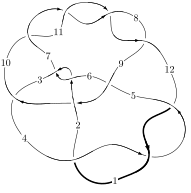
\includegraphics[width=112pt]{../../../GIT/diagram.site/Diagrams/png/1771_12a_0970.png}\\
\ \ \ A knot diagram\footnotemark}&
\allowdisplaybreaks
\textbf{Linearized knot diagam} \\
\cline{2-2}
 &
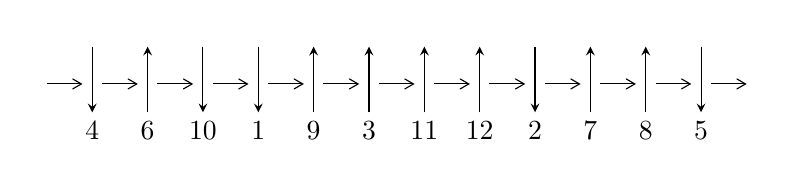
\begin{tikzpicture}[x=20pt, y=17pt]
	% nodes
	\node (C0) at (0, 0) {};
	\node (C1) at (1, 0) {};
	\node (C1U) at (1, +1) {};
	\node (C1D) at (1, -1) {4};

	\node (C2) at (2, 0) {};
	\node (C2U) at (2, +1) {};
	\node (C2D) at (2, -1) {6};

	\node (C3) at (3, 0) {};
	\node (C3U) at (3, +1) {};
	\node (C3D) at (3, -1) {10};

	\node (C4) at (4, 0) {};
	\node (C4U) at (4, +1) {};
	\node (C4D) at (4, -1) {1};

	\node (C5) at (5, 0) {};
	\node (C5U) at (5, +1) {};
	\node (C5D) at (5, -1) {9};

	\node (C6) at (6, 0) {};
	\node (C6U) at (6, +1) {};
	\node (C6D) at (6, -1) {3};

	\node (C7) at (7, 0) {};
	\node (C7U) at (7, +1) {};
	\node (C7D) at (7, -1) {11};

	\node (C8) at (8, 0) {};
	\node (C8U) at (8, +1) {};
	\node (C8D) at (8, -1) {12};

	\node (C9) at (9, 0) {};
	\node (C9U) at (9, +1) {};
	\node (C9D) at (9, -1) {2};

	\node (C10) at (10, 0) {};
	\node (C10U) at (10, +1) {};
	\node (C10D) at (10, -1) {7};

	\node (C11) at (11, 0) {};
	\node (C11U) at (11, +1) {};
	\node (C11D) at (11, -1) {8};

	\node (C12) at (12, 0) {};
	\node (C12U) at (12, +1) {};
	\node (C12D) at (12, -1) {5};
	\node (C13) at (13, 0) {};

	% arrows
	\draw[->,>={angle 60}]
	(C0) edge (C1) (C1) edge (C2) (C2) edge (C3) (C3) edge (C4) (C4) edge (C5) (C5) edge (C6) (C6) edge (C7) (C7) edge (C8) (C8) edge (C9) (C9) edge (C10) (C10) edge (C11) (C11) edge (C12) (C12) edge (C13) ;	\draw[->,>=stealth]
	(C1U) edge (C1D) (C2D) edge (C2U) (C3U) edge (C3D) (C4U) edge (C4D) (C5D) edge (C5U) (C6D) edge (C6U) (C7D) edge (C7U) (C8D) edge (C8U) (C9U) edge (C9D) (C10D) edge (C10U) (C11D) edge (C11U) (C12U) edge (C12D) ;
	\end{tikzpicture} \\
\hhline{~~} \\& 
\textbf{Solving Sequence} \\ \cline{2-2} 
 &
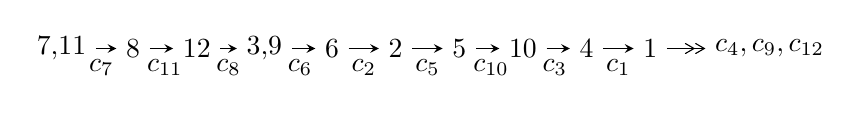
\begin{tikzpicture}[x=23pt, y=7pt]
	% node
	\node (A0) at (-1/8, 0) {7,11};
	\node (A1) at (1, 0) {8};
	\node (A2) at (2, 0) {12};
	\node (A3) at (49/16, 0) {3,9};
	\node (A4) at (33/8, 0) {6};
	\node (A5) at (41/8, 0) {2};
	\node (A6) at (49/8, 0) {5};
	\node (A7) at (57/8, 0) {10};
	\node (A8) at (65/8, 0) {4};
	\node (A9) at (73/8, 0) {1};
	\node (C1) at (1/2, -1) {$c_{7}$};
	\node (C2) at (3/2, -1) {$c_{11}$};
	\node (C3) at (5/2, -1) {$c_{8}$};
	\node (C4) at (29/8, -1) {$c_{6}$};
	\node (C5) at (37/8, -1) {$c_{2}$};
	\node (C6) at (45/8, -1) {$c_{5}$};
	\node (C7) at (53/8, -1) {$c_{10}$};
	\node (C8) at (61/8, -1) {$c_{3}$};
	\node (C9) at (69/8, -1) {$c_{1}$};
	\node (A10) at (11, 0) {$c_{4},c_{9},c_{12}$};

	% edge
	\draw[->,>=stealth]	
	(A0) edge (A1) (A1) edge (A2) (A2) edge (A3) (A3) edge (A4) (A4) edge (A5) (A5) edge (A6) (A6) edge (A7) (A7) edge (A8) (A8) edge (A9) ;
	\draw[->>,>={angle 60}]	
	(A9) edge (A10);
\end{tikzpicture} \\ 

\end{tabular} \\

\footnotetext{
The image of knot diagram is generated by the software ``\textbf{Draw programme}" developed by Andrew Bartholomew(\url{http://www.layer8.co.uk/maths/draw/index.htm\#Running-draw}), where we modified some parts for our purpose(\url{https://github.com/CATsTAILs/LinksPainter}).
}\phantom \\ \newline 
\centering \textbf{Ideals for irreducible components\footnotemark of $X_{\text{par}}$} 
 
\begin{align*}
I^u_{1}&=\langle 
3.53471\times10^{56} u^{58}+1.42360\times10^{57} u^{57}+\cdots+3.93692\times10^{56} b-1.65023\times10^{57},\\
\phantom{I^u_{1}}&\phantom{= \langle  }2.21537\times10^{57} u^{58}+1.28547\times10^{58} u^{57}+\cdots+1.77161\times10^{57} a-5.99824\times10^{58},\;u^{59}+6 u^{58}+\cdots-41 u-9\rangle \\
I^u_{2}&=\langle 
b+3 a+1,\;3 a^2+3 a+1,\;u^2- u-1\rangle \\
I^u_{3}&=\langle 
b+1,\;a^2-4 a+6,\;u+1\rangle \\
I^u_{4}&=\langle 
b-1,\;a+2,\;u+1\rangle \\
\\
\end{align*}
\raggedright * 4 irreducible components of $\dim_{\mathbb{C}}=0$, with total 66 representations.\\
\footnotetext{All coefficients of polynomials are rational numbers. But the coefficients are sometimes approximated in decimal forms when there is not enough margin.}
\newpage
\renewcommand{\arraystretch}{1}
\centering \section*{I. $I^u_{1}= \langle 3.53\times10^{56} u^{58}+1.42\times10^{57} u^{57}+\cdots+3.94\times10^{56} b-1.65\times10^{57},\;2.22\times10^{57} u^{58}+1.29\times10^{58} u^{57}+\cdots+1.77\times10^{57} a-6.00\times10^{58},\;u^{59}+6 u^{58}+\cdots-41 u-9 \rangle$}
\flushleft \textbf{(i) Arc colorings}\\
\begin{tabular}{m{7pt} m{180pt} m{7pt} m{180pt} }
\flushright $a_{7}=$&$\begin{pmatrix}1\\0\end{pmatrix}$ \\
\flushright $a_{11}=$&$\begin{pmatrix}0\\u\end{pmatrix}$ \\
\flushright $a_{8}=$&$\begin{pmatrix}1\\- u^2\end{pmatrix}$ \\
\flushright $a_{12}=$&$\begin{pmatrix}u\\- u^3+u\end{pmatrix}$ \\
\flushright $a_{3}=$&$\begin{pmatrix}-1.25048 u^{58}-7.25590 u^{57}+\cdots+63.0832 u+33.8575\\-0.897836 u^{58}-3.61603 u^{57}+\cdots+16.4208 u+4.19168\end{pmatrix}$ \\
\flushright $a_{9}=$&$\begin{pmatrix}- u^2+1\\u^4-2 u^2\end{pmatrix}$ \\
\flushright $a_{6}=$&$\begin{pmatrix}4.46863 u^{58}+17.9681 u^{57}+\cdots-67.6860 u+1.25189\\-5.38311 u^{58}-23.1424 u^{57}+\cdots+108.980 u+28.8269\end{pmatrix}$ \\
\flushright $a_{2}=$&$\begin{pmatrix}2.90235 u^{58}+13.2229 u^{57}+\cdots-72.6610 u-21.8095\\-2.15803 u^{58}-9.57659 u^{57}+\cdots+48.5315 u+11.5997\end{pmatrix}$ \\
\flushright $a_{5}=$&$\begin{pmatrix}-1.96408 u^{58}-9.62149 u^{57}+\cdots+68.3445 u+30.6108\\3.54462 u^{58}+15.7106 u^{57}+\cdots-88.3461 u-20.9626\end{pmatrix}$ \\
\flushright $a_{10}=$&$\begin{pmatrix}- u\\u\end{pmatrix}$ \\
\flushright $a_{4}=$&$\begin{pmatrix}1.66279 u^{58}+5.41036 u^{57}+\cdots-0.319179 u+15.6956\\-3.81111 u^{58}-16.2823 u^{57}+\cdots+79.8231 u+22.3535\end{pmatrix}$ \\
\flushright $a_{1}=$&$\begin{pmatrix}-3.00291 u^{58}-15.3623 u^{57}+\cdots+118.037 u+39.4455\\1.06867 u^{58}+3.16422 u^{57}+\cdots+9.35768 u+12.0523\end{pmatrix}$\\&\end{tabular}
\flushleft \textbf{(ii) Obstruction class $= -1$}\\~\\
\flushleft \textbf{(iii) Cusp Shapes $= -0.777443 u^{58}+1.97110 u^{57}+\cdots-73.4254 u-32.6128$}\\~\\
\newpage\renewcommand{\arraystretch}{1}
\flushleft \textbf{(iv) u-Polynomials at the component}\newline \\
\begin{tabular}{m{50pt}|m{274pt}}
Crossings & \hspace{64pt}u-Polynomials at each crossing \\
\hline $$\begin{aligned}c_{1},c_{4},c_{12}\end{aligned}$$&$\begin{aligned}
&u^{59}-3 u^{58}+\cdots+8 u^2+2
\end{aligned}$\\
\hline $$\begin{aligned}c_{2},c_{6}\end{aligned}$$&$\begin{aligned}
&u^{59}-4 u^{58}+\cdots-19 u+3
\end{aligned}$\\
\hline $$\begin{aligned}c_{3}\end{aligned}$$&$\begin{aligned}
&9(9 u^{59}+48 u^{58}+\cdots-422003 u+85781)
\end{aligned}$\\
\hline $$\begin{aligned}c_{5}\end{aligned}$$&$\begin{aligned}
&9(9 u^{59}-75 u^{58}+\cdots-1270890 u-386003)
\end{aligned}$\\
\hline $$\begin{aligned}c_{7},c_{8},c_{10}\\c_{11}\end{aligned}$$&$\begin{aligned}
&u^{59}-6 u^{58}+\cdots-41 u+9
\end{aligned}$\\
\hline $$\begin{aligned}c_{9}\end{aligned}$$&$\begin{aligned}
&u^{59}-2 u^{58}+\cdots-1152 u+432
\end{aligned}$\\
\hline
\end{tabular}\\~\\
\newpage\renewcommand{\arraystretch}{1}
\flushleft \textbf{(v) Riley Polynomials at the component}\newline \\
\begin{tabular}{m{50pt}|m{274pt}}
Crossings & \hspace{64pt}Riley Polynomials at each crossing \\
\hline $$\begin{aligned}c_{1},c_{4},c_{12}\end{aligned}$$&$\begin{aligned}
&y^{59}+63 y^{58}+\cdots-32 y-4
\end{aligned}$\\
\hline $$\begin{aligned}c_{2},c_{6}\end{aligned}$$&$\begin{aligned}
&y^{59}-44 y^{58}+\cdots+355 y-9
\end{aligned}$\\
\hline $$\begin{aligned}c_{3}\end{aligned}$$&$\begin{aligned}
&81(81 y^{59}+1944 y^{58}+\cdots+1.62773\times10^{10} y-7.35838\times10^{9})
\end{aligned}$\\
\hline $$\begin{aligned}c_{5}\end{aligned}$$&$\begin{aligned}
&81(81 y^{59}-5643 y^{58}+\cdots+5.63820\times10^{12} y-1.48998\times10^{11})
\end{aligned}$\\
\hline $$\begin{aligned}c_{7},c_{8},c_{10}\\c_{11}\end{aligned}$$&$\begin{aligned}
&y^{59}-76 y^{58}+\cdots+1483 y-81
\end{aligned}$\\
\hline $$\begin{aligned}c_{9}\end{aligned}$$&$\begin{aligned}
&y^{59}+22 y^{58}+\cdots-1627776 y-186624
\end{aligned}$\\
\hline
\end{tabular}\\~\\
\newpage\flushleft \textbf{(vi) Complex Volumes and Cusp Shapes}
$$\begin{array}{c|c|c}  
\text{Solutions to }I^u_{1}& \I (\text{vol} + \sqrt{-1}CS) & \text{Cusp shape}\\
 \hline 
\begin{aligned}
u &= -0.857889 + 0.543473 I \\
a &= -0.935537 - 1.008220 I \\
b &= \phantom{-}1.210920 + 0.035673 I\end{aligned}
 & \phantom{-}4.74114 - 0.35952 I & \phantom{-0.000000 } 0 \\ \hline\begin{aligned}
u &= -0.857889 - 0.543473 I \\
a &= -0.935537 + 1.008220 I \\
b &= \phantom{-}1.210920 - 0.035673 I\end{aligned}
 & \phantom{-}4.74114 + 0.35952 I & \phantom{-0.000000 } 0 \\ \hline\begin{aligned}
u &= -0.130615 + 0.967990 I \\
a &= \phantom{-}0.190514 + 0.374185 I \\
b &= -1.318690 + 0.257478 I\end{aligned}
 & \phantom{-}9.56415 - 6.01109 I & \phantom{-0.000000 } 0 \\ \hline\begin{aligned}
u &= -0.130615 - 0.967990 I \\
a &= \phantom{-}0.190514 - 0.374185 I \\
b &= -1.318690 - 0.257478 I\end{aligned}
 & \phantom{-}9.56415 + 6.01109 I & \phantom{-0.000000 } 0 \\ \hline\begin{aligned}
u &= \phantom{-}0.948364 + 0.213838 I \\
a &= \phantom{-}1.51212 - 0.71166 I \\
b &= -1.37230 - 0.44609 I\end{aligned}
 & \phantom{-}5.43776 + 2.93026 I & \phantom{-0.000000 } 0 \\ \hline\begin{aligned}
u &= \phantom{-}0.948364 - 0.213838 I \\
a &= \phantom{-}1.51212 + 0.71166 I \\
b &= -1.37230 + 0.44609 I\end{aligned}
 & \phantom{-}5.43776 - 2.93026 I & \phantom{-0.000000 } 0 \\ \hline\begin{aligned}
u &= \phantom{-}0.960664 + 0.374018 I \\
a &= -0.305542 + 0.131521 I \\
b &= \phantom{-}0.126556 + 0.984052 I\end{aligned}
 & \phantom{-}8.38003 + 6.19609 I & \phantom{-0.000000 } 0 \\ \hline\begin{aligned}
u &= \phantom{-}0.960664 - 0.374018 I \\
a &= -0.305542 - 0.131521 I \\
b &= \phantom{-}0.126556 - 0.984052 I\end{aligned}
 & \phantom{-}8.38003 - 6.19609 I & \phantom{-0.000000 } 0 \\ \hline\begin{aligned}
u &= \phantom{-}0.969759 + 0.438458 I \\
a &= -1.42805 + 0.92716 I \\
b &= \phantom{-}1.37512 + 0.41779 I\end{aligned}
 & \phantom{-}5.94572 + 7.83644 I & \phantom{-0.000000 } 0 \\ \hline\begin{aligned}
u &= \phantom{-}0.969759 - 0.438458 I \\
a &= -1.42805 - 0.92716 I \\
b &= \phantom{-}1.37512 - 0.41779 I\end{aligned}
 & \phantom{-}5.94572 - 7.83644 I & \phantom{-0.000000 } 0\\
 \hline 
 \end{array}$$\newpage$$\begin{array}{c|c|c}  
\text{Solutions to }I^u_{1}& \I (\text{vol} + \sqrt{-1}CS) & \text{Cusp shape}\\
 \hline 
\begin{aligned}
u &= \phantom{-}1.066870 + 0.057775 I \\
a &= -1.208650 - 0.520306 I \\
b &= \phantom{-}1.291030 - 0.498774 I\end{aligned}
 & \phantom{-}11.99040 + 0.77771 I & \phantom{-0.000000 } 0 \\ \hline\begin{aligned}
u &= \phantom{-}1.066870 - 0.057775 I \\
a &= -1.208650 + 0.520306 I \\
b &= \phantom{-}1.291030 + 0.498774 I\end{aligned}
 & \phantom{-}11.99040 - 0.77771 I & \phantom{-0.000000 } 0 \\ \hline\begin{aligned}
u &= -0.764641 + 0.343047 I \\
a &= \phantom{-}1.330310 - 0.471171 I \\
b &= \phantom{-}0.362348 + 0.017749 I\end{aligned}
 & \phantom{-}6.96622 - 0.49717 I & \phantom{-}6.23462 + 1.41414 I \\ \hline\begin{aligned}
u &= -0.764641 - 0.343047 I \\
a &= \phantom{-}1.330310 + 0.471171 I \\
b &= \phantom{-}0.362348 - 0.017749 I\end{aligned}
 & \phantom{-}6.96622 + 0.49717 I & \phantom{-}6.23462 - 1.41414 I \\ \hline\begin{aligned}
u &= \phantom{-}0.799754 + 0.143772 I \\
a &= \phantom{-}0.272317 + 0.190800 I \\
b &= -0.120952 - 1.081830 I\end{aligned}
 & \phantom{-}1.12793 + 2.71854 I & \phantom{-}10.64746 - 8.72932 I \\ \hline\begin{aligned}
u &= \phantom{-}0.799754 - 0.143772 I \\
a &= \phantom{-}0.272317 - 0.190800 I \\
b &= -0.120952 + 1.081830 I\end{aligned}
 & \phantom{-}1.12793 - 2.71854 I & \phantom{-}10.64746 + 8.72932 I \\ \hline\begin{aligned}
u &= \phantom{-}1.046220 + 0.597660 I \\
a &= \phantom{-}1.28813 - 0.95719 I \\
b &= -1.38493 - 0.42023 I\end{aligned}
 & \phantom{-}13.1773 + 11.1774 I & \phantom{-0.000000 } 0 \\ \hline\begin{aligned}
u &= \phantom{-}1.046220 - 0.597660 I \\
a &= \phantom{-}1.28813 + 0.95719 I \\
b &= -1.38493 + 0.42023 I\end{aligned}
 & \phantom{-}13.1773 - 11.1774 I & \phantom{-0.000000 } 0 \\ \hline\begin{aligned}
u &= -1.21103\phantom{ +0.000000I} \\
a &= -1.33100\phantom{ +0.000000I} \\
b &= \phantom{-}0.716569\phantom{ +0.000000I}\end{aligned}
 & \phantom{-}2.64173\phantom{ +0.000000I} & \phantom{-0.000000 } 0 \\ \hline\begin{aligned}
u &= -0.732538\phantom{ +0.000000I} \\
a &= \phantom{-}4.79896\phantom{ +0.000000I} \\
b &= -1.05042\phantom{ +0.000000I}\end{aligned}
 & \phantom{-}2.92652\phantom{ +0.000000I} & -31.4710\phantom{ +0.000000I}\\
 \hline 
 \end{array}$$\newpage$$\begin{array}{c|c|c}  
\text{Solutions to }I^u_{1}& \I (\text{vol} + \sqrt{-1}CS) & \text{Cusp shape}\\
 \hline 
\begin{aligned}
u &= -0.118101 + 0.722024 I \\
a &= \phantom{-}0.086917 - 0.358660 I \\
b &= \phantom{-}1.229760 - 0.250070 I\end{aligned}
 & \phantom{-}2.59101 - 3.95881 I & \phantom{-}6.03862 + 7.13057 I \\ \hline\begin{aligned}
u &= -0.118101 - 0.722024 I \\
a &= \phantom{-}0.086917 + 0.358660 I \\
b &= \phantom{-}1.229760 + 0.250070 I\end{aligned}
 & \phantom{-}2.59101 + 3.95881 I & \phantom{-}6.03862 - 7.13057 I \\ \hline\begin{aligned}
u &= -0.986283 + 0.810419 I \\
a &= \phantom{-}0.787138 + 0.653314 I \\
b &= -1.331550 - 0.064088 I\end{aligned}
 & \phantom{-}11.99500 + 0.09773 I & \phantom{-0.000000 } 0 \\ \hline\begin{aligned}
u &= -0.986283 - 0.810419 I \\
a &= \phantom{-}0.787138 - 0.653314 I \\
b &= -1.331550 + 0.064088 I\end{aligned}
 & \phantom{-}11.99500 - 0.09773 I & \phantom{-0.000000 } 0 \\ \hline\begin{aligned}
u &= -0.622166 + 0.142096 I \\
a &= -0.610096 + 0.520870 I \\
b &= -0.136025 + 0.091898 I\end{aligned}
 & \phantom{-}1.150150 - 0.364893 I & \phantom{-}8.81978 + 0.27517 I \\ \hline\begin{aligned}
u &= -0.622166 - 0.142096 I \\
a &= -0.610096 - 0.520870 I \\
b &= -0.136025 - 0.091898 I\end{aligned}
 & \phantom{-}1.150150 + 0.364893 I & \phantom{-}8.81978 - 0.27517 I \\ \hline\begin{aligned}
u &= -0.117244 + 0.612352 I \\
a &= \phantom{-}0.812578 - 0.945370 I \\
b &= \phantom{-}0.134811 - 0.595483 I\end{aligned}
 & \phantom{-}5.05432 - 2.85507 I & \phantom{-}3.39383 + 3.61710 I \\ \hline\begin{aligned}
u &= -0.117244 - 0.612352 I \\
a &= \phantom{-}0.812578 + 0.945370 I \\
b &= \phantom{-}0.134811 + 0.595483 I\end{aligned}
 & \phantom{-}5.05432 + 2.85507 I & \phantom{-}3.39383 - 3.61710 I \\ \hline\begin{aligned}
u &= -1.400890 + 0.081228 I \\
a &= \phantom{-}1.207210 + 0.357135 I \\
b &= -0.851572 - 0.540881 I\end{aligned}
 & \phantom{-}6.44938 + 2.04861 I & \phantom{-0.000000 } 0 \\ \hline\begin{aligned}
u &= -1.400890 - 0.081228 I \\
a &= \phantom{-}1.207210 - 0.357135 I \\
b &= -0.851572 + 0.540881 I\end{aligned}
 & \phantom{-}6.44938 - 2.04861 I & \phantom{-0.000000 } 0\\
 \hline 
 \end{array}$$\newpage$$\begin{array}{c|c|c}  
\text{Solutions to }I^u_{1}& \I (\text{vol} + \sqrt{-1}CS) & \text{Cusp shape}\\
 \hline 
\begin{aligned}
u &= -0.420938 + 0.095647 I \\
a &= \phantom{-}3.99493 + 4.99920 I \\
b &= \phantom{-}0.990001 + 0.115515 I\end{aligned}
 & \phantom{-}7.27721 - 0.14920 I & \phantom{-}10.48371 - 3.97631 I \\ \hline\begin{aligned}
u &= -0.420938 - 0.095647 I \\
a &= \phantom{-}3.99493 - 4.99920 I \\
b &= \phantom{-}0.990001 - 0.115515 I\end{aligned}
 & \phantom{-}7.27721 + 0.14920 I & \phantom{-}10.48371 + 3.97631 I \\ \hline\begin{aligned}
u &= \phantom{-}0.392846 + 0.073015 I \\
a &= \phantom{-}1.305270 + 0.430518 I \\
b &= -0.582701 - 0.749020 I\end{aligned}
 & \phantom{-}0.63593 + 2.21296 I & -5.75964 - 6.65166 I \\ \hline\begin{aligned}
u &= \phantom{-}0.392846 - 0.073015 I \\
a &= \phantom{-}1.305270 - 0.430518 I \\
b &= -0.582701 + 0.749020 I\end{aligned}
 & \phantom{-}0.63593 - 2.21296 I & -5.75964 + 6.65166 I \\ \hline\begin{aligned}
u &= -0.195055 + 0.340133 I \\
a &= -1.55948 + 0.68613 I \\
b &= -1.091800 + 0.185883 I\end{aligned}
 & \phantom{-}1.98756 - 0.99917 I & \phantom{-}2.40222 - 1.62487 I \\ \hline\begin{aligned}
u &= -0.195055 - 0.340133 I \\
a &= -1.55948 - 0.68613 I \\
b &= -1.091800 - 0.185883 I\end{aligned}
 & \phantom{-}1.98756 + 0.99917 I & \phantom{-}2.40222 + 1.62487 I \\ \hline\begin{aligned}
u &= \phantom{-}1.61129 + 0.03030 I \\
a &= -0.088005 - 0.279498 I \\
b &= -0.217256 - 0.380886 I\end{aligned}
 & \phantom{-}8.95456 + 0.95974 I & \phantom{-0.000000 } 0 \\ \hline\begin{aligned}
u &= \phantom{-}1.61129 - 0.03030 I \\
a &= -0.088005 + 0.279498 I \\
b &= -0.217256 + 0.380886 I\end{aligned}
 & \phantom{-}8.95456 - 0.95974 I & \phantom{-0.000000 } 0 \\ \hline\begin{aligned}
u &= \phantom{-}0.068702 + 0.357326 I \\
a &= -1.24232 + 0.82388 I \\
b &= \phantom{-}0.092635 + 0.542344 I\end{aligned}
 & -0.908481 - 0.907750 I & -3.97873 + 3.36038 I \\ \hline\begin{aligned}
u &= \phantom{-}0.068702 - 0.357326 I \\
a &= -1.24232 - 0.82388 I \\
b &= \phantom{-}0.092635 - 0.542344 I\end{aligned}
 & -0.908481 + 0.907750 I & -3.97873 - 3.36038 I\\
 \hline 
 \end{array}$$\newpage$$\begin{array}{c|c|c}  
\text{Solutions to }I^u_{1}& \I (\text{vol} + \sqrt{-1}CS) & \text{Cusp shape}\\
 \hline 
\begin{aligned}
u &= \phantom{-}1.66142\phantom{ +0.000000I} \\
a &= \phantom{-}2.81188\phantom{ +0.000000I} \\
b &= -1.21634\phantom{ +0.000000I}\end{aligned}
 & \phantom{-}11.4761\phantom{ +0.000000I} & \phantom{-0.000000 } 0 \\ \hline\begin{aligned}
u &= \phantom{-}1.67528 + 0.06502 I \\
a &= \phantom{-}0.057515 + 0.457143 I \\
b &= \phantom{-}0.454603 + 0.532651 I\end{aligned}
 & \phantom{-}15.6369 + 1.8583 I & \phantom{-0.000000 } 0 \\ \hline\begin{aligned}
u &= \phantom{-}1.67528 - 0.06502 I \\
a &= \phantom{-}0.057515 - 0.457143 I \\
b &= \phantom{-}0.454603 - 0.532651 I\end{aligned}
 & \phantom{-}15.6369 - 1.8583 I & \phantom{-0.000000 } 0 \\ \hline\begin{aligned}
u &= -1.67823 + 0.03059 I \\
a &= \phantom{-}0.178129 - 0.749329 I \\
b &= -0.101652 + 1.402470 I\end{aligned}
 & \phantom{-}9.97496 - 3.33073 I & \phantom{-0.000000 } 0 \\ \hline\begin{aligned}
u &= -1.67823 - 0.03059 I \\
a &= \phantom{-}0.178129 + 0.749329 I \\
b &= -0.101652 - 1.402470 I\end{aligned}
 & \phantom{-}9.97496 + 3.33073 I & \phantom{-0.000000 } 0 \\ \hline\begin{aligned}
u &= \phantom{-}1.69183 + 0.11419 I \\
a &= -1.87237 + 0.56142 I \\
b &= \phantom{-}1.315370 + 0.125779 I\end{aligned}
 & \phantom{-}13.68640 + 2.79097 I & \phantom{-0.000000 } 0 \\ \hline\begin{aligned}
u &= \phantom{-}1.69183 - 0.11419 I \\
a &= -1.87237 - 0.56142 I \\
b &= \phantom{-}1.315370 - 0.125779 I\end{aligned}
 & \phantom{-}13.68640 - 2.79097 I & \phantom{-0.000000 } 0 \\ \hline\begin{aligned}
u &= -1.70433 + 0.05549 I \\
a &= \phantom{-}1.94975 + 0.14139 I \\
b &= -1.56251 + 0.59298 I\end{aligned}
 & \phantom{-}14.8568 - 3.9980 I & \phantom{-0.000000 } 0 \\ \hline\begin{aligned}
u &= -1.70433 - 0.05549 I \\
a &= \phantom{-}1.94975 - 0.14139 I \\
b &= -1.56251 - 0.59298 I\end{aligned}
 & \phantom{-}14.8568 + 3.9980 I & \phantom{-0.000000 } 0 \\ \hline\begin{aligned}
u &= -1.70709 + 0.09794 I \\
a &= -0.304137 + 0.494271 I \\
b &= \phantom{-}0.119151 - 1.247520 I\end{aligned}
 & \phantom{-}17.7739 - 8.0669 I & \phantom{-0.000000 } 0\\
 \hline 
 \end{array}$$\newpage$$\begin{array}{c|c|c}  
\text{Solutions to }I^u_{1}& \I (\text{vol} + \sqrt{-1}CS) & \text{Cusp shape}\\
 \hline 
\begin{aligned}
u &= -1.70709 - 0.09794 I \\
a &= -0.304137 - 0.494271 I \\
b &= \phantom{-}0.119151 + 1.247520 I\end{aligned}
 & \phantom{-}17.7739 + 8.0669 I & \phantom{-0.000000 } 0 \\ \hline\begin{aligned}
u &= -1.70726 + 0.11689 I \\
a &= -1.95829 - 0.38629 I \\
b &= \phantom{-}1.51361 - 0.53501 I\end{aligned}
 & \phantom{-}15.3175 - 10.0440 I & \phantom{-0.000000 } 0 \\ \hline\begin{aligned}
u &= -1.70726 - 0.11689 I \\
a &= -1.95829 + 0.38629 I \\
b &= \phantom{-}1.51361 + 0.53501 I\end{aligned}
 & \phantom{-}15.3175 + 10.0440 I & \phantom{-0.000000 } 0 \\ \hline\begin{aligned}
u &= -1.73066 + 0.01255 I \\
a &= -1.72454 - 0.03435 I \\
b &= \phantom{-}1.50767 + 0.66940 I\end{aligned}
 & -17.4675 - 1.0530 I & \phantom{-0.000000 } 0 \\ \hline\begin{aligned}
u &= -1.73066 - 0.01255 I \\
a &= -1.72454 + 0.03435 I \\
b &= \phantom{-}1.50767 - 0.66940 I\end{aligned}
 & -17.4675 + 1.0530 I & \phantom{-0.000000 } 0 \\ \hline\begin{aligned}
u &= -1.73213 + 0.16868 I \\
a &= \phantom{-}1.84723 + 0.54357 I \\
b &= -1.46340 + 0.53545 I\end{aligned}
 & -16.6726 - 14.3095 I & \phantom{-0.000000 } 0 \\ \hline\begin{aligned}
u &= -1.73213 - 0.16868 I \\
a &= \phantom{-}1.84723 - 0.54357 I \\
b &= -1.46340 - 0.53545 I\end{aligned}
 & -16.6726 + 14.3095 I & \phantom{-0.000000 } 0 \\ \hline\begin{aligned}
u &= \phantom{-}1.78302 + 0.21856 I \\
a &= \phantom{-}1.55482 - 0.43122 I \\
b &= -1.41314 - 0.15182 I\end{aligned}
 & -17.8772 + 4.1906 I & \phantom{-0.000000 } 0 \\ \hline\begin{aligned}
u &= \phantom{-}1.78302 - 0.21856 I \\
a &= \phantom{-}1.55482 + 0.43122 I \\
b &= -1.41314 + 0.15182 I\end{aligned}
 & -17.8772 - 4.1906 I & \phantom{-0.000000 } 0\\
 \hline 
 \end{array}$$\newpage\newpage\renewcommand{\arraystretch}{1}
\centering \section*{II. $I^u_{2}= \langle b+3 a+1,\;3 a^2+3 a+1,\;u^2- u-1 \rangle$}
\flushleft \textbf{(i) Arc colorings}\\
\begin{tabular}{m{7pt} m{180pt} m{7pt} m{180pt} }
\flushright $a_{7}=$&$\begin{pmatrix}1\\0\end{pmatrix}$ \\
\flushright $a_{11}=$&$\begin{pmatrix}0\\u\end{pmatrix}$ \\
\flushright $a_{8}=$&$\begin{pmatrix}1\\- u-1\end{pmatrix}$ \\
\flushright $a_{12}=$&$\begin{pmatrix}u\\- u-1\end{pmatrix}$ \\
\flushright $a_{3}=$&$\begin{pmatrix}a\\-3 a-1\end{pmatrix}$ \\
\flushright $a_{9}=$&$\begin{pmatrix}- u\\u\end{pmatrix}$ \\
\flushright $a_{6}=$&$\begin{pmatrix}2 a+2\\-3 a-2\end{pmatrix}$ \\
\flushright $a_{2}=$&$\begin{pmatrix}3 a\\-3 a\end{pmatrix}$ \\
\flushright $a_{5}=$&$\begin{pmatrix}a u+3 a+2\\- a u-4 a-2\end{pmatrix}$ \\
\flushright $a_{10}=$&$\begin{pmatrix}- u\\u\end{pmatrix}$ \\
\flushright $a_{4}=$&$\begin{pmatrix}2 a u+3 a+u+1\\-2 a u-5 a- u-2\end{pmatrix}$ \\
\flushright $a_{1}=$&$\begin{pmatrix}- a u+3 a+1\\a u-2 a-1\end{pmatrix}$\\&\end{tabular}
\flushleft \textbf{(ii) Obstruction class $= 1$}\\~\\
\flushleft \textbf{(iii) Cusp Shapes $= 10 a u-5 a+\frac{11}{3} u+\frac{26}{3}$}\\~\\
\newpage\renewcommand{\arraystretch}{1}
\flushleft \textbf{(iv) u-Polynomials at the component}\newline \\
\begin{tabular}{m{50pt}|m{274pt}}
Crossings & \hspace{64pt}u-Polynomials at each crossing \\
\hline $$\begin{aligned}c_{1},c_{6},c_{12}\end{aligned}$$&$\begin{aligned}
&(u^2- u+1)^2
\end{aligned}$\\
\hline $$\begin{aligned}c_{2},c_{4}\end{aligned}$$&$\begin{aligned}
&(u^2+u+1)^2
\end{aligned}$\\
\hline $$\begin{aligned}c_{3}\end{aligned}$$&$\begin{aligned}
&9(9 u^4+9 u^2+1)
\end{aligned}$\\
\hline $$\begin{aligned}c_{5}\end{aligned}$$&$\begin{aligned}
&9(9 u^4-9 u^3+3 u+1)
\end{aligned}$\\
\hline $$\begin{aligned}c_{7},c_{8}\end{aligned}$$&$\begin{aligned}
&(u^2- u-1)^2
\end{aligned}$\\
\hline $$\begin{aligned}c_{9}\end{aligned}$$&$\begin{aligned}
&u^4
\end{aligned}$\\
\hline $$\begin{aligned}c_{10},c_{11}\end{aligned}$$&$\begin{aligned}
&(u^2+u-1)^2
\end{aligned}$\\
\hline
\end{tabular}\\~\\
\newpage\renewcommand{\arraystretch}{1}
\flushleft \textbf{(v) Riley Polynomials at the component}\newline \\
\begin{tabular}{m{50pt}|m{274pt}}
Crossings & \hspace{64pt}Riley Polynomials at each crossing \\
\hline $$\begin{aligned}c_{1},c_{2},c_{4}\\c_{6},c_{12}\end{aligned}$$&$\begin{aligned}
&(y^2+y+1)^2
\end{aligned}$\\
\hline $$\begin{aligned}c_{3}\end{aligned}$$&$\begin{aligned}
&81(9 y^2+9 y+1)^2
\end{aligned}$\\
\hline $$\begin{aligned}c_{5}\end{aligned}$$&$\begin{aligned}
&81(81 y^4-81 y^3+72 y^2-9 y+1)
\end{aligned}$\\
\hline $$\begin{aligned}c_{7},c_{8},c_{10}\\c_{11}\end{aligned}$$&$\begin{aligned}
&(y^2-3 y+1)^2
\end{aligned}$\\
\hline $$\begin{aligned}c_{9}\end{aligned}$$&$\begin{aligned}
&y^4
\end{aligned}$\\
\hline
\end{tabular}\\~\\
\newpage\flushleft \textbf{(vi) Complex Volumes and Cusp Shapes}
$$\begin{array}{c|c|c}  
\text{Solutions to }I^u_{2}& \I (\text{vol} + \sqrt{-1}CS) & \text{Cusp shape}\\
 \hline 
\begin{aligned}
u &= -0.618034\phantom{ +0.000000I} \\
a &= -0.500000 + 0.288675 I \\
b &= \phantom{-}0.500000 - 0.866025 I\end{aligned}
 & \phantom{-}0.98696 - 2.02988 I & \phantom{-}11.99071 - 3.22749 I \\ \hline\begin{aligned}
u &= -0.618034\phantom{ +0.000000I} \\
a &= -0.500000 - 0.288675 I \\
b &= \phantom{-}0.500000 + 0.866025 I\end{aligned}
 & \phantom{-}0.98696 + 2.02988 I & \phantom{-}11.99071 + 3.22749 I \\ \hline\begin{aligned}
u &= \phantom{-}1.61803\phantom{ +0.000000I} \\
a &= -0.500000 + 0.288675 I \\
b &= \phantom{-}0.500000 - 0.866025 I\end{aligned}
 & \phantom{-}8.88264 - 2.02988 I & \phantom{-}9.00929 + 3.22749 I \\ \hline\begin{aligned}
u &= \phantom{-}1.61803\phantom{ +0.000000I} \\
a &= -0.500000 - 0.288675 I \\
b &= \phantom{-}0.500000 + 0.866025 I\end{aligned}
 & \phantom{-}8.88264 + 2.02988 I & \phantom{-}9.00929 - 3.22749 I\\
 \hline 
 \end{array}$$\newpage\newpage\renewcommand{\arraystretch}{1}
\centering \section*{III. $I^u_{3}= \langle b+1,\;a^2-4 a+6,\;u+1 \rangle$}
\flushleft \textbf{(i) Arc colorings}\\
\begin{tabular}{m{7pt} m{180pt} m{7pt} m{180pt} }
\flushright $a_{7}=$&$\begin{pmatrix}1\\0\end{pmatrix}$ \\
\flushright $a_{11}=$&$\begin{pmatrix}0\\-1\end{pmatrix}$ \\
\flushright $a_{8}=$&$\begin{pmatrix}1\\-1\end{pmatrix}$ \\
\flushright $a_{12}=$&$\begin{pmatrix}-1\\0\end{pmatrix}$ \\
\flushright $a_{3}=$&$\begin{pmatrix}a\\-1\end{pmatrix}$ \\
\flushright $a_{9}=$&$\begin{pmatrix}0\\-1\end{pmatrix}$ \\
\flushright $a_{6}=$&$\begin{pmatrix}- a+1\\1\end{pmatrix}$ \\
\flushright $a_{2}=$&$\begin{pmatrix}1\\0\end{pmatrix}$ \\
\flushright $a_{5}=$&$\begin{pmatrix}- a+1\\- a+2\end{pmatrix}$ \\
\flushright $a_{10}=$&$\begin{pmatrix}1\\-1\end{pmatrix}$ \\
\flushright $a_{4}=$&$\begin{pmatrix}1\\a-2\end{pmatrix}$ \\
\flushright $a_{1}=$&$\begin{pmatrix}- a+3\\2\end{pmatrix}$\\&\end{tabular}
\flushleft \textbf{(ii) Obstruction class $= 1$}\\~\\
\flushleft \textbf{(iii) Cusp Shapes $= 12$}\\~\\
\newpage\renewcommand{\arraystretch}{1}
\flushleft \textbf{(iv) u-Polynomials at the component}\newline \\
\begin{tabular}{m{50pt}|m{274pt}}
Crossings & \hspace{64pt}u-Polynomials at each crossing \\
\hline $$\begin{aligned}c_{1},c_{4},c_{12}\end{aligned}$$&$\begin{aligned}
&u^2+2
\end{aligned}$\\
\hline $$\begin{aligned}c_{2},c_{9},c_{10}\\c_{11}\end{aligned}$$&$\begin{aligned}
&(u-1)^2
\end{aligned}$\\
\hline $$\begin{aligned}c_{3}\end{aligned}$$&$\begin{aligned}
&u^2+2 u+3
\end{aligned}$\\
\hline $$\begin{aligned}c_{5}\end{aligned}$$&$\begin{aligned}
&u^2-2 u+3
\end{aligned}$\\
\hline $$\begin{aligned}c_{6},c_{7},c_{8}\end{aligned}$$&$\begin{aligned}
&(u+1)^2
\end{aligned}$\\
\hline
\end{tabular}\\~\\
\newpage\renewcommand{\arraystretch}{1}
\flushleft \textbf{(v) Riley Polynomials at the component}\newline \\
\begin{tabular}{m{50pt}|m{274pt}}
Crossings & \hspace{64pt}Riley Polynomials at each crossing \\
\hline $$\begin{aligned}c_{1},c_{4},c_{12}\end{aligned}$$&$\begin{aligned}
&(y+2)^2
\end{aligned}$\\
\hline $$\begin{aligned}c_{2},c_{6},c_{7}\\c_{8},c_{9},c_{10}\\c_{11}\end{aligned}$$&$\begin{aligned}
&(y-1)^2
\end{aligned}$\\
\hline $$\begin{aligned}c_{3},c_{5}\end{aligned}$$&$\begin{aligned}
&y^2+2 y+9
\end{aligned}$\\
\hline
\end{tabular}\\~\\
\newpage\flushleft \textbf{(vi) Complex Volumes and Cusp Shapes}
$$\begin{array}{c|c|c}  
\text{Solutions to }I^u_{3}& \I (\text{vol} + \sqrt{-1}CS) & \text{Cusp shape}\\
 \hline 
\begin{aligned}
u &= -1.00000\phantom{ +0.000000I} \\
a &= \phantom{-}2.00000 + 1.41421 I \\
b &= -1.00000\phantom{ +0.000000I}\end{aligned}
 & \phantom{-}8.22467\phantom{ +0.000000I} & \phantom{-}12.0000\phantom{ +0.000000I} \\ \hline\begin{aligned}
u &= -1.00000\phantom{ +0.000000I} \\
a &= \phantom{-}2.00000 - 1.41421 I \\
b &= -1.00000\phantom{ +0.000000I}\end{aligned}
 & \phantom{-}8.22467\phantom{ +0.000000I} & \phantom{-}12.0000\phantom{ +0.000000I}\\
 \hline 
 \end{array}$$\newpage\newpage\renewcommand{\arraystretch}{1}
\centering \section*{IV. $I^u_{4}= \langle b-1,\;a+2,\;u+1 \rangle$}
\flushleft \textbf{(i) Arc colorings}\\
\begin{tabular}{m{7pt} m{180pt} m{7pt} m{180pt} }
\flushright $a_{7}=$&$\begin{pmatrix}1\\0\end{pmatrix}$ \\
\flushright $a_{11}=$&$\begin{pmatrix}0\\-1\end{pmatrix}$ \\
\flushright $a_{8}=$&$\begin{pmatrix}1\\-1\end{pmatrix}$ \\
\flushright $a_{12}=$&$\begin{pmatrix}-1\\0\end{pmatrix}$ \\
\flushright $a_{3}=$&$\begin{pmatrix}-2\\1\end{pmatrix}$ \\
\flushright $a_{9}=$&$\begin{pmatrix}0\\-1\end{pmatrix}$ \\
\flushright $a_{6}=$&$\begin{pmatrix}-1\\1\end{pmatrix}$ \\
\flushright $a_{2}=$&$\begin{pmatrix}-1\\0\end{pmatrix}$ \\
\flushright $a_{5}=$&$\begin{pmatrix}-1\\0\end{pmatrix}$ \\
\flushright $a_{10}=$&$\begin{pmatrix}1\\-1\end{pmatrix}$ \\
\flushright $a_{4}=$&$\begin{pmatrix}-1\\0\end{pmatrix}$ \\
\flushright $a_{1}=$&$\begin{pmatrix}-1\\0\end{pmatrix}$\\&\end{tabular}
\flushleft \textbf{(ii) Obstruction class $= 1$}\\~\\
\flushleft \textbf{(iii) Cusp Shapes $= 12$}\\~\\
\newpage\renewcommand{\arraystretch}{1}
\flushleft \textbf{(iv) u-Polynomials at the component}\newline \\
\begin{tabular}{m{50pt}|m{274pt}}
Crossings & \hspace{64pt}u-Polynomials at each crossing \\
\hline $$\begin{aligned}c_{1},c_{4},c_{12}\end{aligned}$$&$\begin{aligned}
&u
\end{aligned}$\\
\hline $$\begin{aligned}c_{2},c_{7},c_{8}\\c_{9}\end{aligned}$$&$\begin{aligned}
&u+1
\end{aligned}$\\
\hline $$\begin{aligned}c_{3},c_{5},c_{6}\\c_{10},c_{11}\end{aligned}$$&$\begin{aligned}
&u-1
\end{aligned}$\\
\hline
\end{tabular}\\~\\
\newpage\renewcommand{\arraystretch}{1}
\flushleft \textbf{(v) Riley Polynomials at the component}\newline \\
\begin{tabular}{m{50pt}|m{274pt}}
Crossings & \hspace{64pt}Riley Polynomials at each crossing \\
\hline $$\begin{aligned}c_{1},c_{4},c_{12}\end{aligned}$$&$\begin{aligned}
&y
\end{aligned}$\\
\hline $$\begin{aligned}c_{2},c_{3},c_{5}\\c_{6},c_{7},c_{8}\\c_{9},c_{10},c_{11}\end{aligned}$$&$\begin{aligned}
&y-1
\end{aligned}$\\
\hline
\end{tabular}\\~\\
\newpage\flushleft \textbf{(vi) Complex Volumes and Cusp Shapes}
$$\begin{array}{c|c|c}  
\text{Solutions to }I^u_{4}& \I (\text{vol} + \sqrt{-1}CS) & \text{Cusp shape}\\
 \hline 
\begin{aligned}
u &= -1.00000\phantom{ +0.000000I} \\
a &= -2.00000\phantom{ +0.000000I} \\
b &= \phantom{-}1.00000\phantom{ +0.000000I}\end{aligned}
 & \phantom{-}3.28987\phantom{ +0.000000I} & \phantom{-}12.0000\phantom{ +0.000000I}\\
 \hline 
 \end{array}$$\newpage
\newpage\renewcommand{\arraystretch}{1}
\centering \section*{ V. u-Polynomials}
\begin{tabular}{m{50pt}|m{274pt}}
Crossings & \hspace{64pt}u-Polynomials at each crossing \\
\hline $$\begin{aligned}c_{1},c_{12}\end{aligned}$$&$\begin{aligned}
&u(u^2+2)(u^2- u+1)^2(u^{59}-3 u^{58}+\cdots+8 u^{2}+2)
\end{aligned}$\\
\hline $$\begin{aligned}c_{2}\end{aligned}$$&$\begin{aligned}
&((u-1)^2)(u+1)(u^2+u+1)^2(u^{59}-4 u^{58}+\cdots-19 u+3)
\end{aligned}$\\
\hline $$\begin{aligned}c_{3}\end{aligned}$$&$\begin{aligned}
&81(u-1)(u^2+2 u+3)(9 u^4+9 u^2+1)\\
&\cdot(9 u^{59}+48 u^{58}+\cdots-422003 u+85781)
\end{aligned}$\\
\hline $$\begin{aligned}c_{4}\end{aligned}$$&$\begin{aligned}
&u(u^2+2)(u^2+u+1)^2(u^{59}-3 u^{58}+\cdots+8 u^{2}+2)
\end{aligned}$\\
\hline $$\begin{aligned}c_{5}\end{aligned}$$&$\begin{aligned}
&81(u-1)(u^2-2 u+3)(9 u^4-9 u^3+3 u+1)\\
&\cdot(9 u^{59}-75 u^{58}+\cdots-1270890 u-386003)
\end{aligned}$\\
\hline $$\begin{aligned}c_{6}\end{aligned}$$&$\begin{aligned}
&(u-1)(u+1)^2(u^2- u+1)^2(u^{59}-4 u^{58}+\cdots-19 u+3)
\end{aligned}$\\
\hline $$\begin{aligned}c_{7},c_{8}\end{aligned}$$&$\begin{aligned}
&((u+1)^3)(u^2- u-1)^2(u^{59}-6 u^{58}+\cdots-41 u+9)
\end{aligned}$\\
\hline $$\begin{aligned}c_{9}\end{aligned}$$&$\begin{aligned}
&u^4(u-1)^2(u+1)(u^{59}-2 u^{58}+\cdots-1152 u+432)
\end{aligned}$\\
\hline $$\begin{aligned}c_{10},c_{11}\end{aligned}$$&$\begin{aligned}
&((u-1)^3)(u^2+u-1)^2(u^{59}-6 u^{58}+\cdots-41 u+9)
\end{aligned}$\\
\hline
\end{tabular}\newpage\renewcommand{\arraystretch}{1}
\centering \section*{ VI. Riley Polynomials}
\begin{tabular}{m{50pt}|m{274pt}}
Crossings & \hspace{64pt}Riley Polynomials at each crossing \\
\hline $$\begin{aligned}c_{1},c_{4},c_{12}\end{aligned}$$&$\begin{aligned}
&y(y+2)^2(y^2+y+1)^2(y^{59}+63 y^{58}+\cdots-32 y-4)
\end{aligned}$\\
\hline $$\begin{aligned}c_{2},c_{6}\end{aligned}$$&$\begin{aligned}
&((y-1)^3)(y^2+y+1)^2(y^{59}-44 y^{58}+\cdots+355 y-9)
\end{aligned}$\\
\hline $$\begin{aligned}c_{3}\end{aligned}$$&$\begin{aligned}
&6561(y-1)(y^2+2 y+9)(9 y^2+9 y+1)^2\\
&\cdot(81 y^{59}+1944 y^{58}+\cdots+16277317023 y-7358379961)
\end{aligned}$\\
\hline $$\begin{aligned}c_{5}\end{aligned}$$&$\begin{aligned}
&6561(y-1)(y^2+2 y+9)(81 y^4-81 y^3+72 y^2-9 y+1)\\
&\cdot(81 y^{59}-5643 y^{58}+\cdots+5638201231006 y-148998316009)
\end{aligned}$\\
\hline $$\begin{aligned}c_{7},c_{8},c_{10}\\c_{11}\end{aligned}$$&$\begin{aligned}
&((y-1)^3)(y^2-3 y+1)^2(y^{59}-76 y^{58}+\cdots+1483 y-81)
\end{aligned}$\\
\hline $$\begin{aligned}c_{9}\end{aligned}$$&$\begin{aligned}
&y^4(y-1)^3(y^{59}+22 y^{58}+\cdots-1627776 y-186624)
\end{aligned}$\\
\hline
\end{tabular}
\vskip 2pc
\end{document}